\documentclass{beamer}
\usepackage[utf8]{inputenc}
\usepackage[english]{babel}
\usepackage{amsmath}
\usepackage{amsthm}
\usepackage{amssymb}
\usepackage{fancyhdr}
\usepackage{setspace}
\usepackage{graphicx}
\usepackage{colortbl}
\usepackage{tikz}
\usepackage{pgf}
\usepackage{subcaption}
\usepackage{listings}
\usepackage{indentfirst}

\makeatletter
\renewcommand{\@biblabel}[1]{#1.}
\makeatother

\addtobeamertemplate{navigation symbols}{}{%
    \usebeamerfont{footline}%
    \usebeamercolor[fg]{footline}%
    \hspace{1em}%
    \insertframenumber/\inserttotalframenumber
}

\setbeamertemplate{bibliography item}[text]
\mode<presentation> {

\usetheme[compress]{Singapore}
\usecolortheme{orchid}
}

\setcounter{tocdepth}{1}


\useinnertheme{rounded}
\let\oldfootnote\footnote
\renewcommand\footnote[1][]{\oldfootnote[frame,#1]}

\usepackage{graphicx}

%----------------------------------------------------------------------------------------
%	TITLE PAGE
%----------------------------------------------------------------------------------------

\title{Adversarial Attacks on Cross-lingual Models}

\author{Birshert Alexey}
\date{\today}

\begin{document}

\begin{frame}
\titlepage
\end{frame}

\setbeamertemplate{section in toc}{\inserttocsectionnumber.~\inserttocsection}
\setbeamertemplate{subsection in toc}{\qquad~\inserttocsubsection\par}
\setbeamerfont{subsection in toc}{size=\tiny}

%------------------------------------------------
\section{INTRODUCTION}
%------------------------------------------------

\begin{frame}
\frametitle{Code-switching}
\begin{figure}
	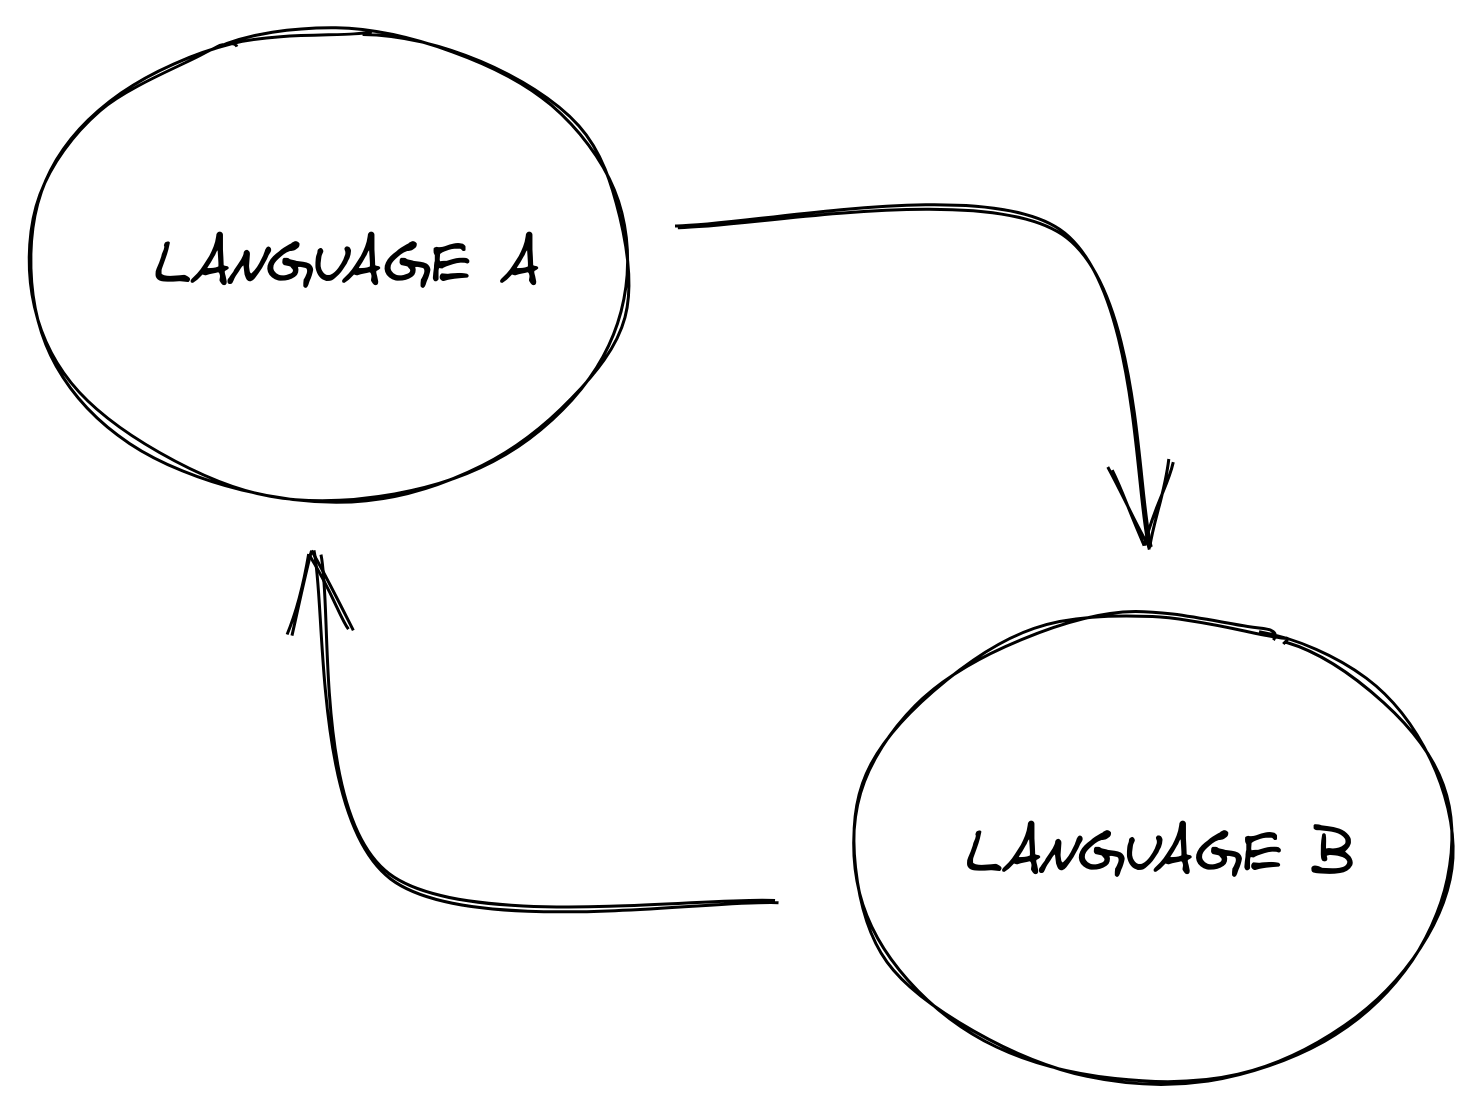
\includegraphics[width=0.8\linewidth]{images/1.png}
\end{figure}
\end{frame}

%------------------------------------------------

\begin{frame}
\frametitle{Texts with code-switching generation}
\begin{figure}
	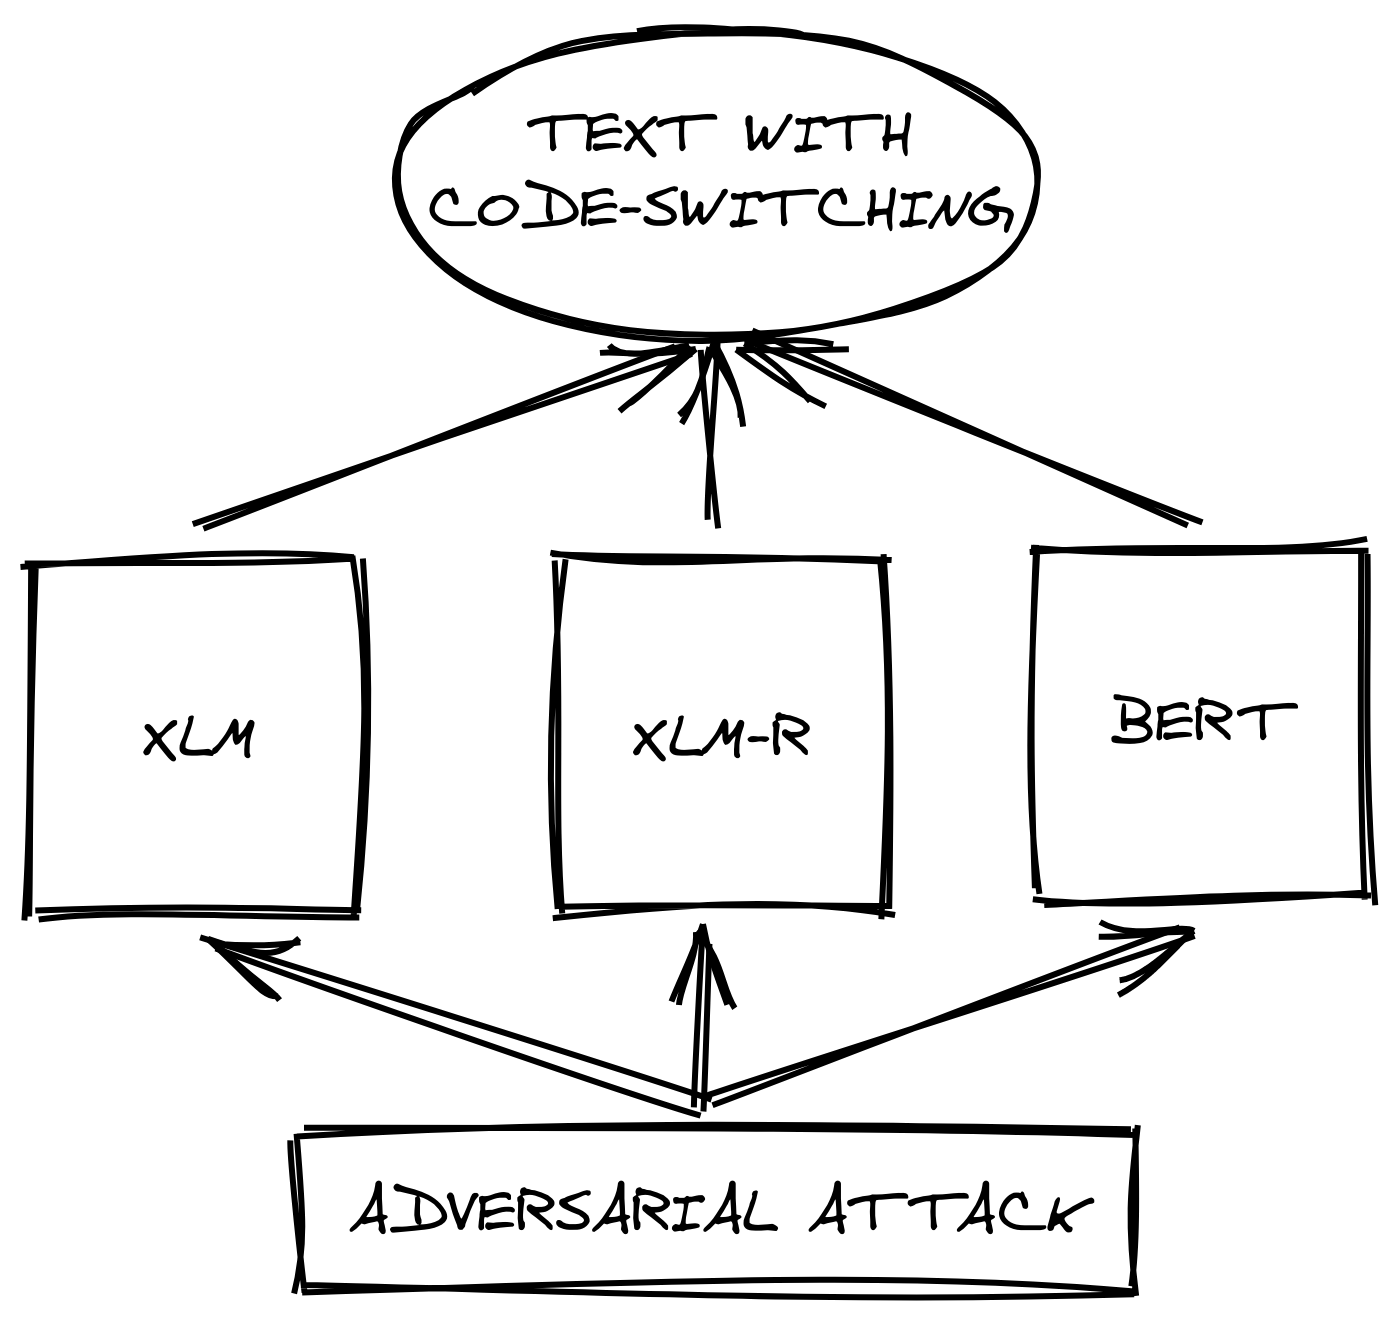
\includegraphics[width=0.7\linewidth]{images/3.png}
\end{figure}
\end{frame}

%------------------------------------------------

%------------------------------------------------
\section{METHODS}
%------------------------------------------------

\begin{frame}
\frametitle{Training procces}
\begin{figure}
	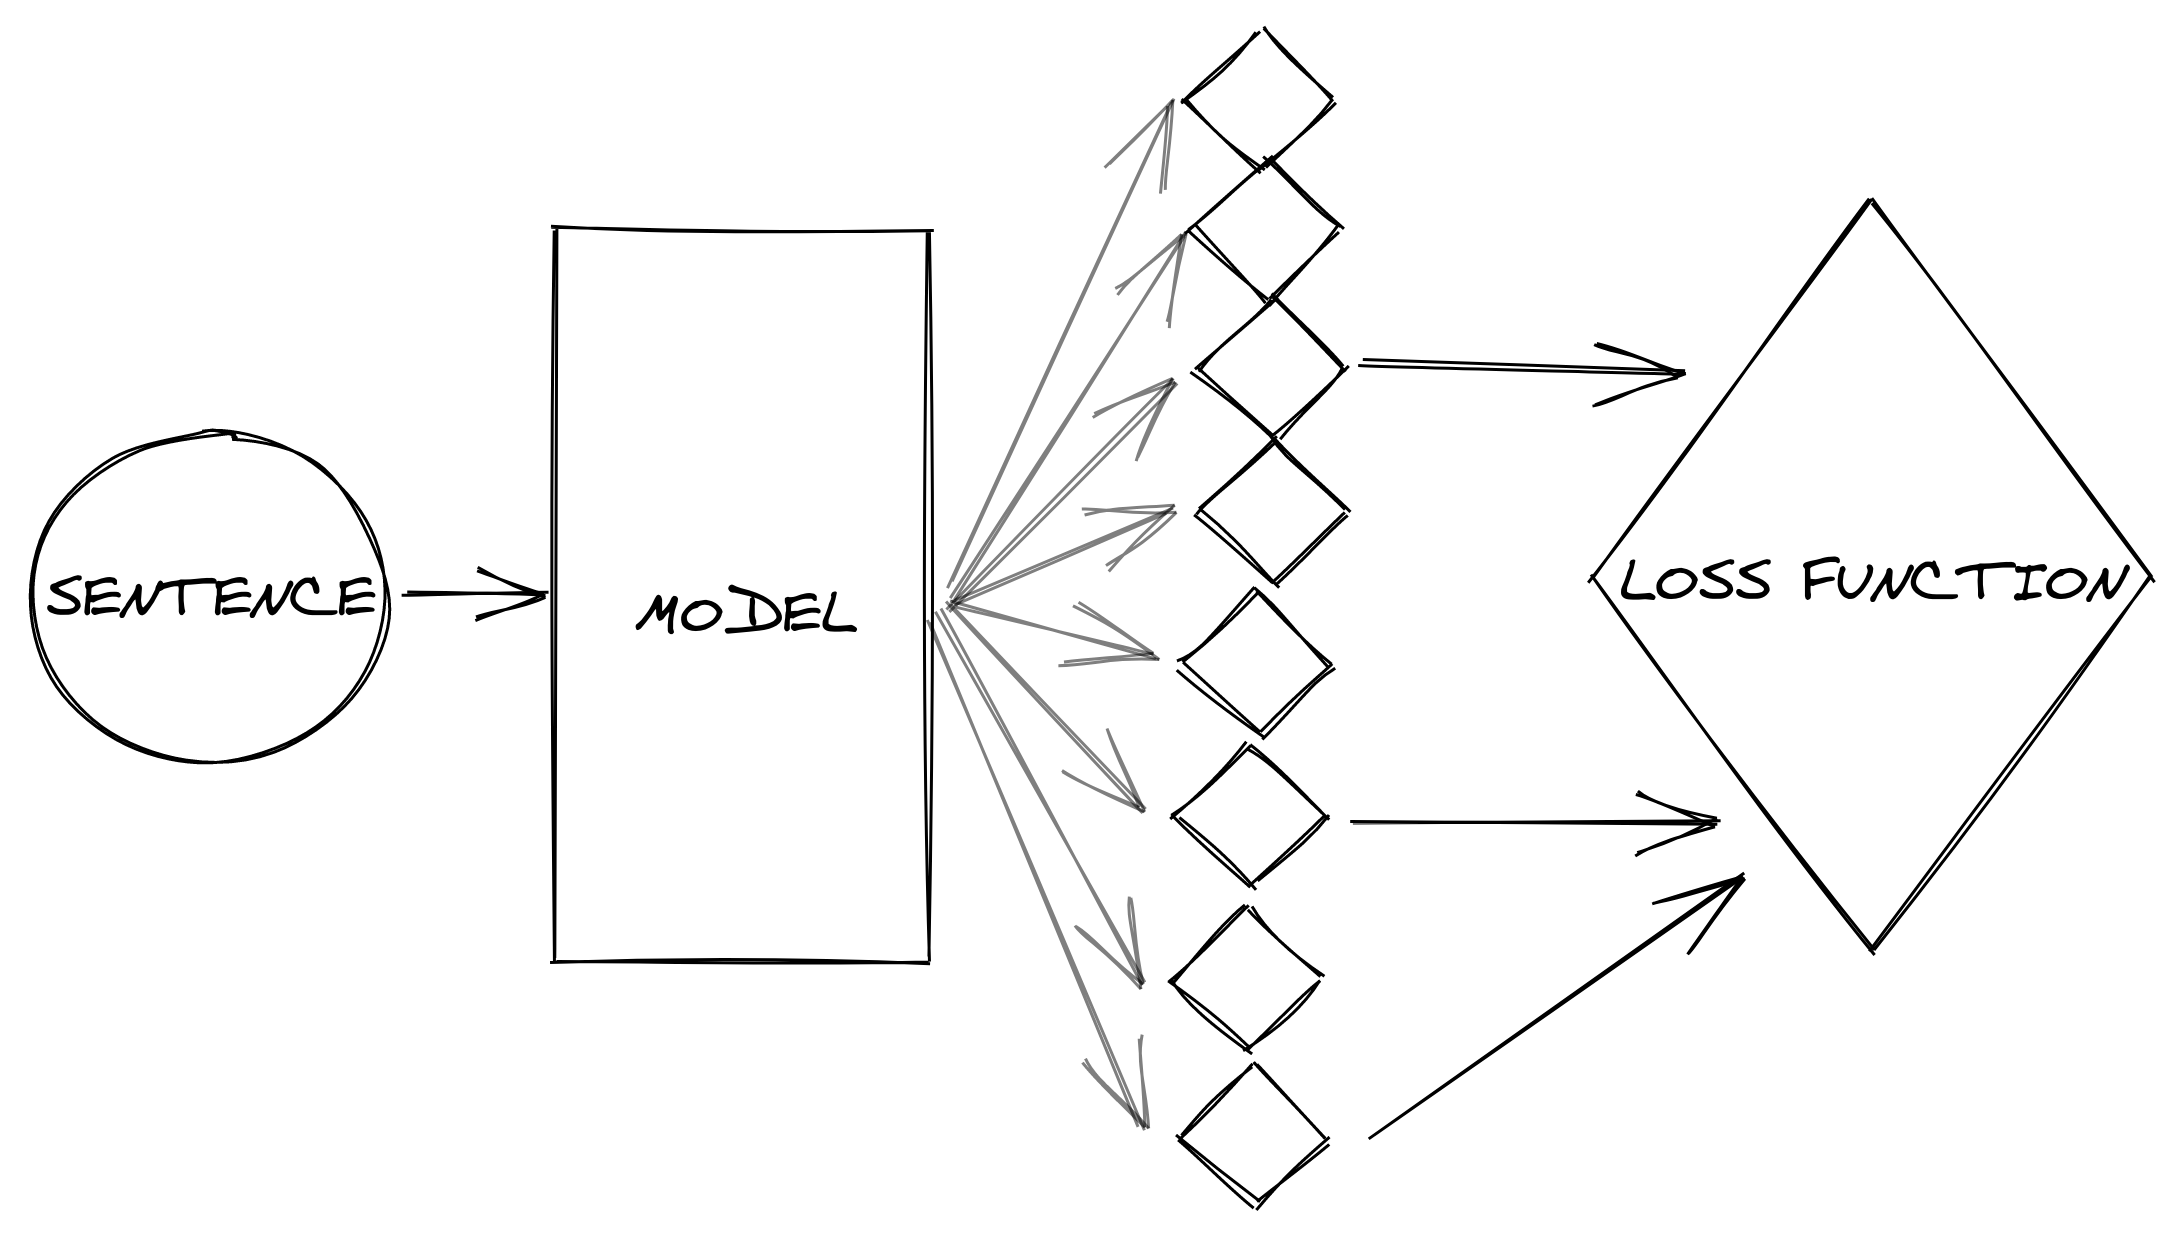
\includegraphics[width=0.9\linewidth]{images/4.png}
\end{figure}
\end{frame}

%------------------------------------------------

\begin{frame}
\frametitle{Training procces}
\begin{figure}
	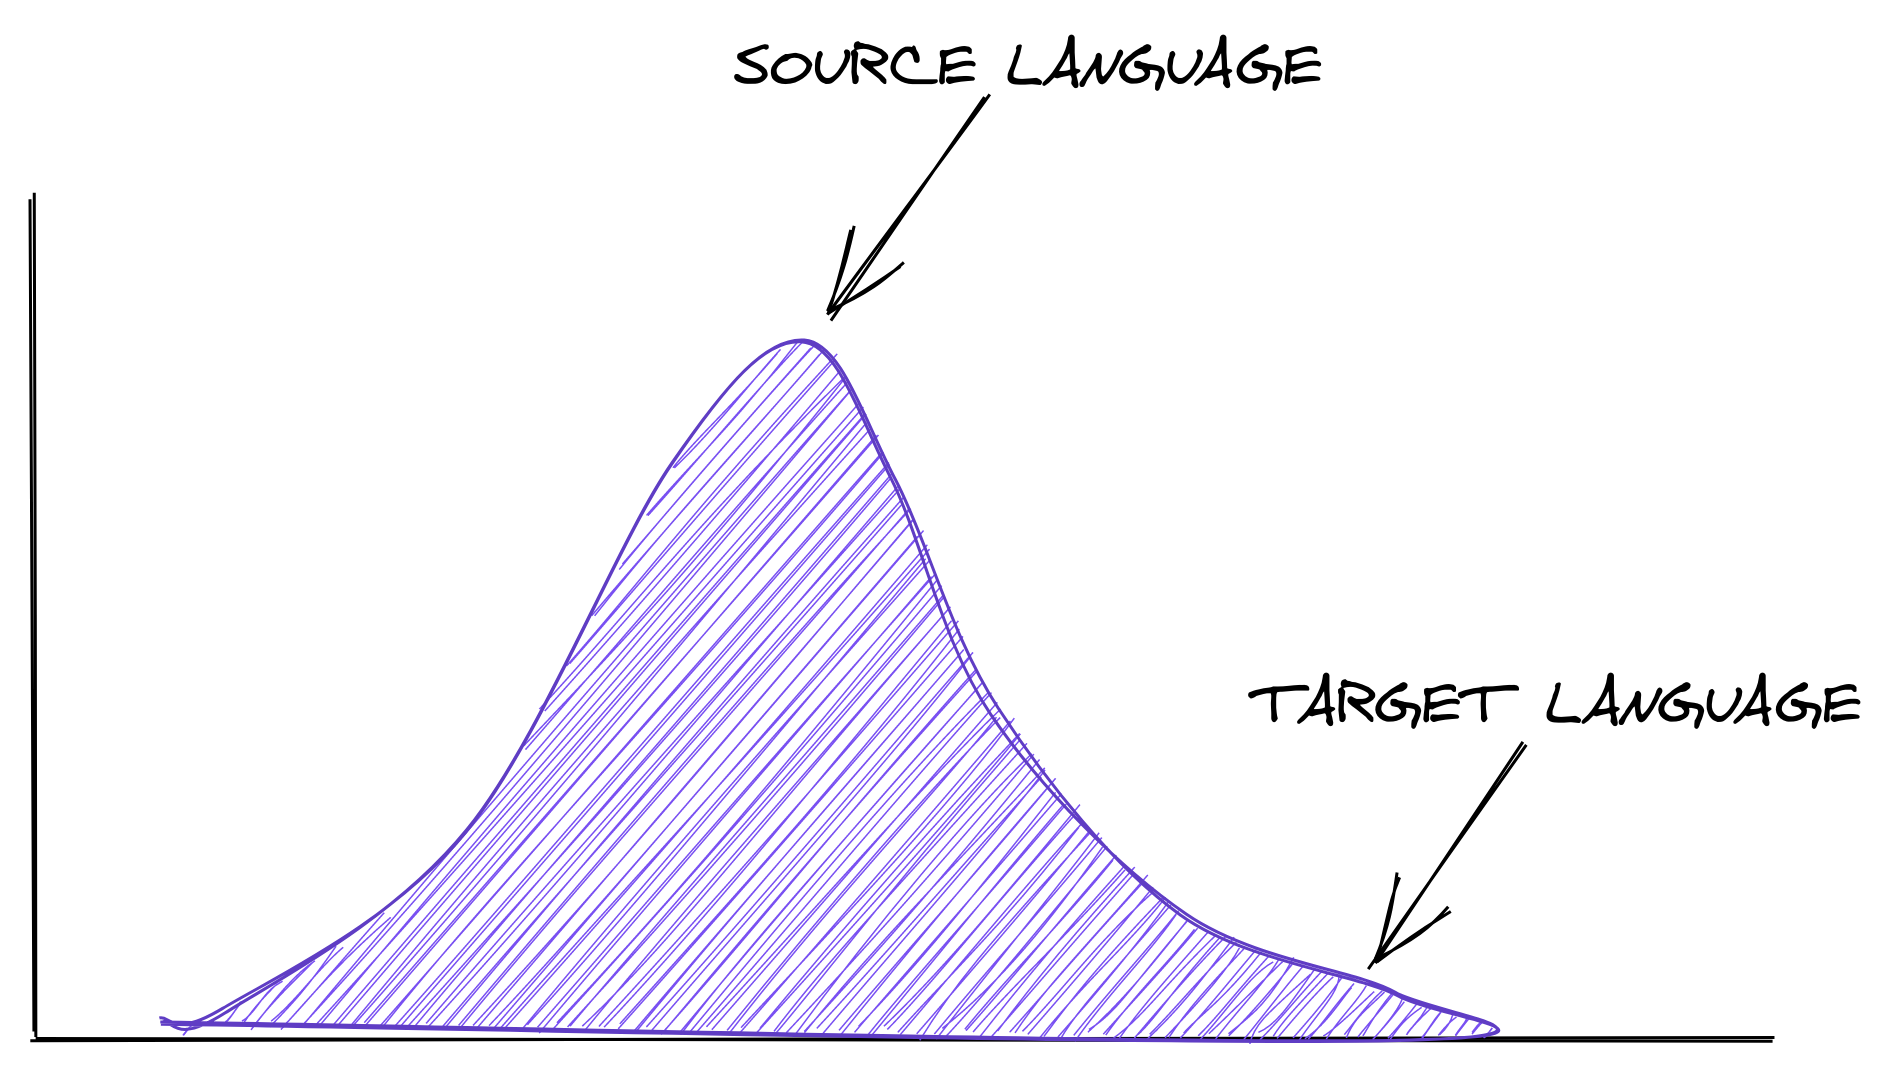
\includegraphics[width=0.9\linewidth]{images/7.png}
\end{figure}
\end{frame}

%------------------------------------------------

\begin{frame}
\frametitle{Training procces}
\begin{figure}
	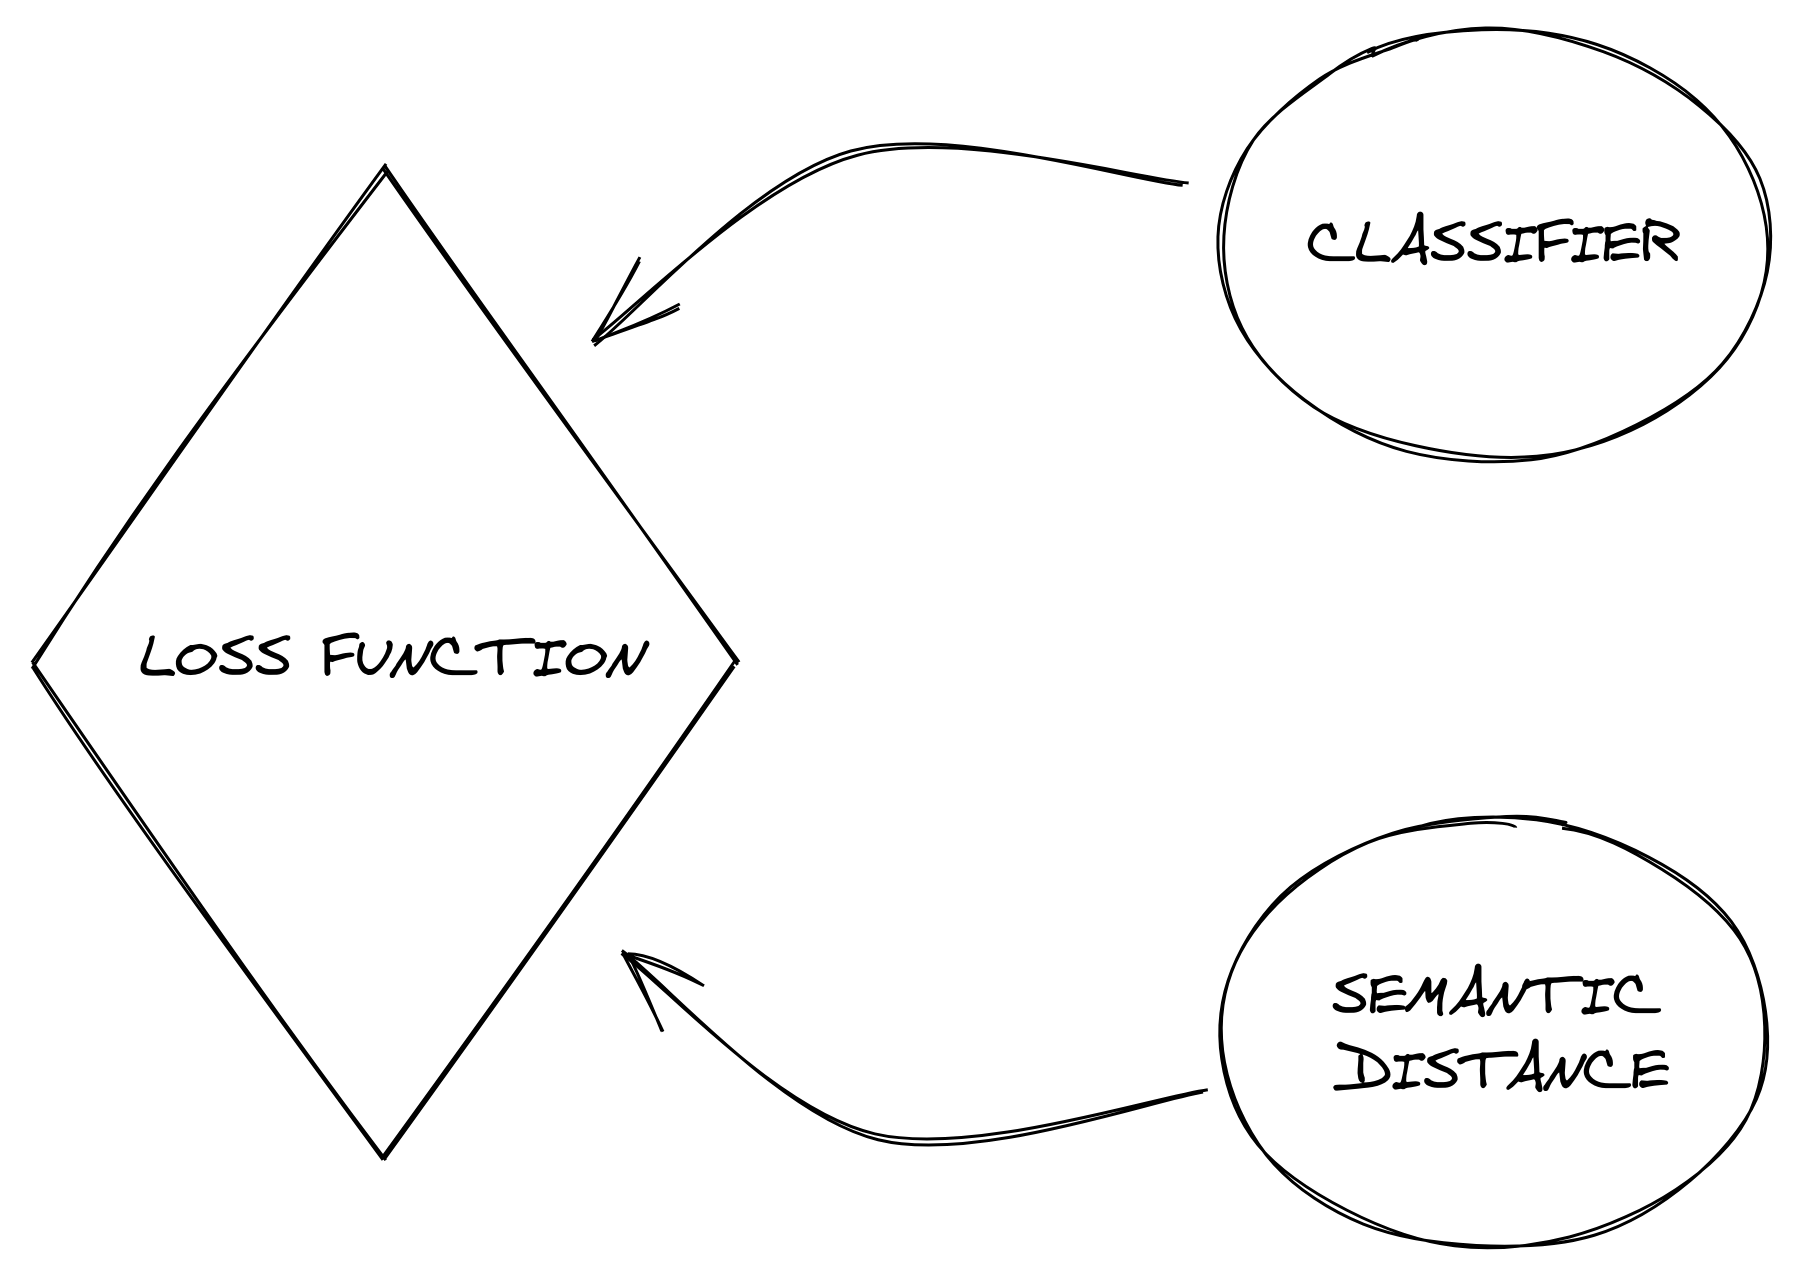
\includegraphics[width=0.9\linewidth]{images/5.png}
\end{figure}
\end{frame}

%------------------------------------------------

\begin{frame}
\frametitle{Experiments}
\begin{figure}
	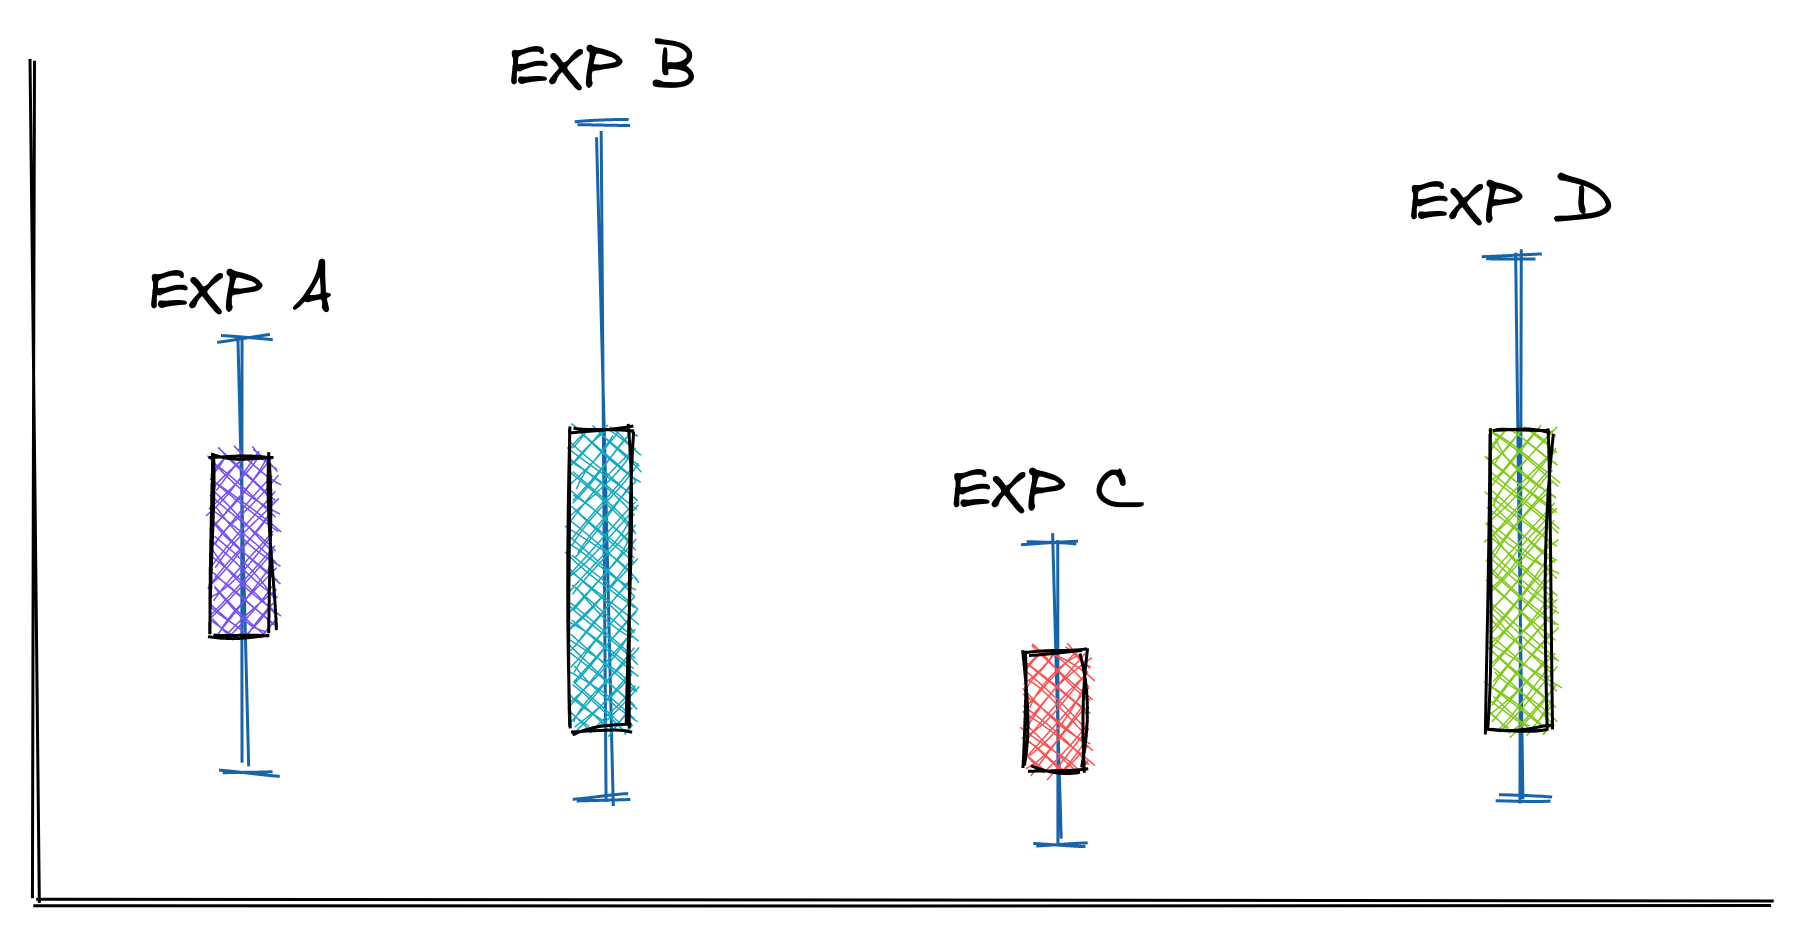
\includegraphics[width=0.9\linewidth]{images/2.png}
\end{figure}
\end{frame}

%------------------------------------------------

\begin{frame}
\frametitle{Evaluation}
\begin{figure}
	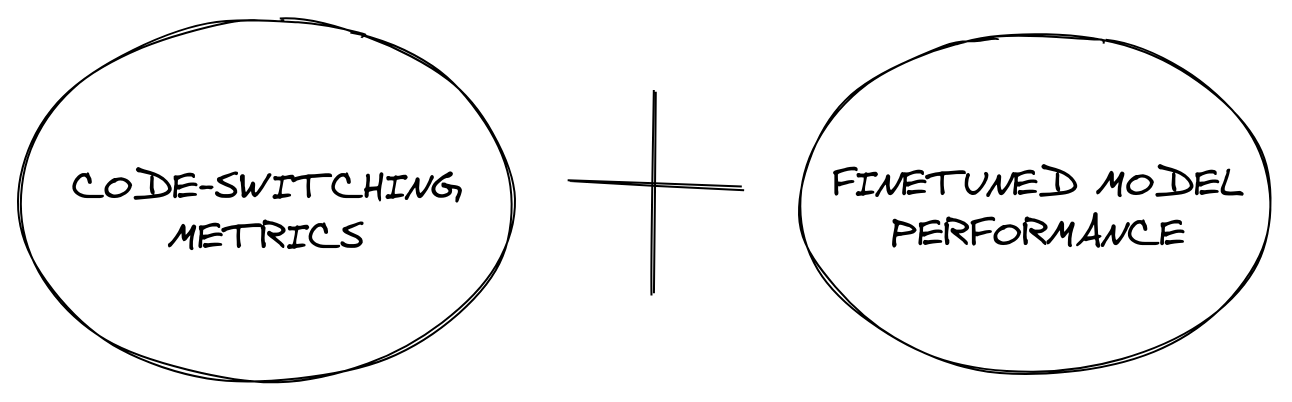
\includegraphics[width=0.9\linewidth]{images/6.png}
\end{figure}
\end{frame}

%------------------------------------------------

%------------------------------------------------
\section{RESULTS ANTICIPATED}
%------------------------------------------------

\begin{frame}
\begin{figure}
	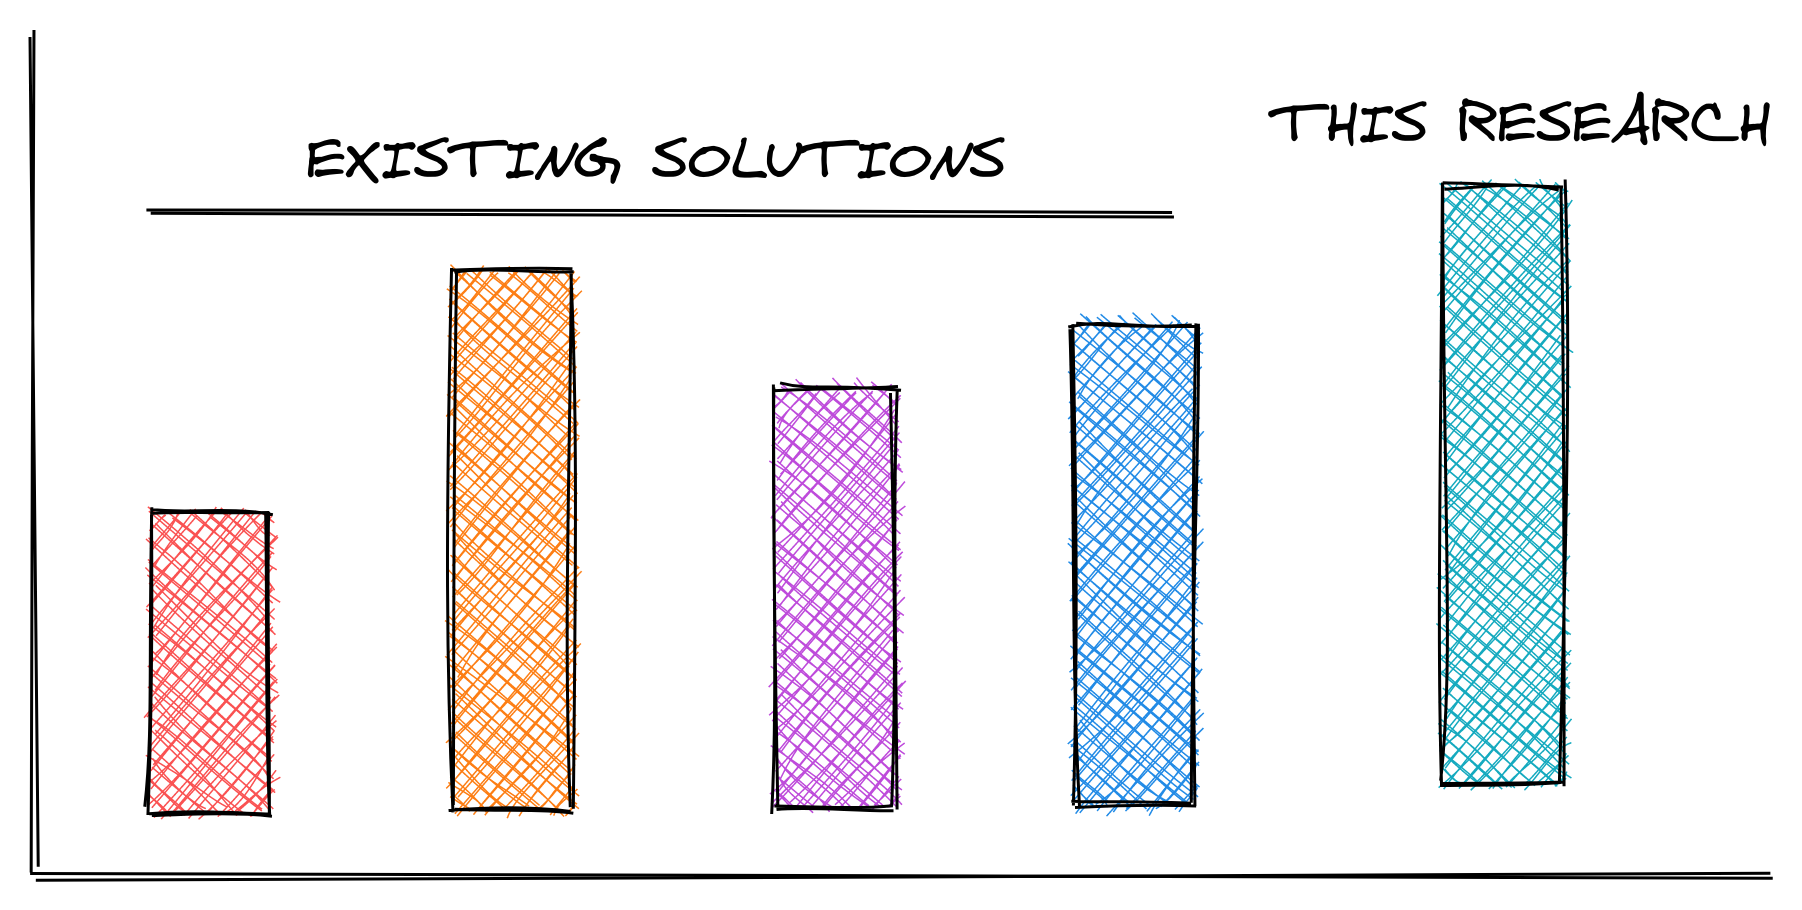
\includegraphics[width=0.9\linewidth]{images/8.png}
\end{figure}
\end{frame}

%------------------------------------------------

%------------------------------------------------
\section{CONCLUSION}
%------------------------------------------------

\begin{frame}
\frametitle{Future plans}
\begin{figure}
	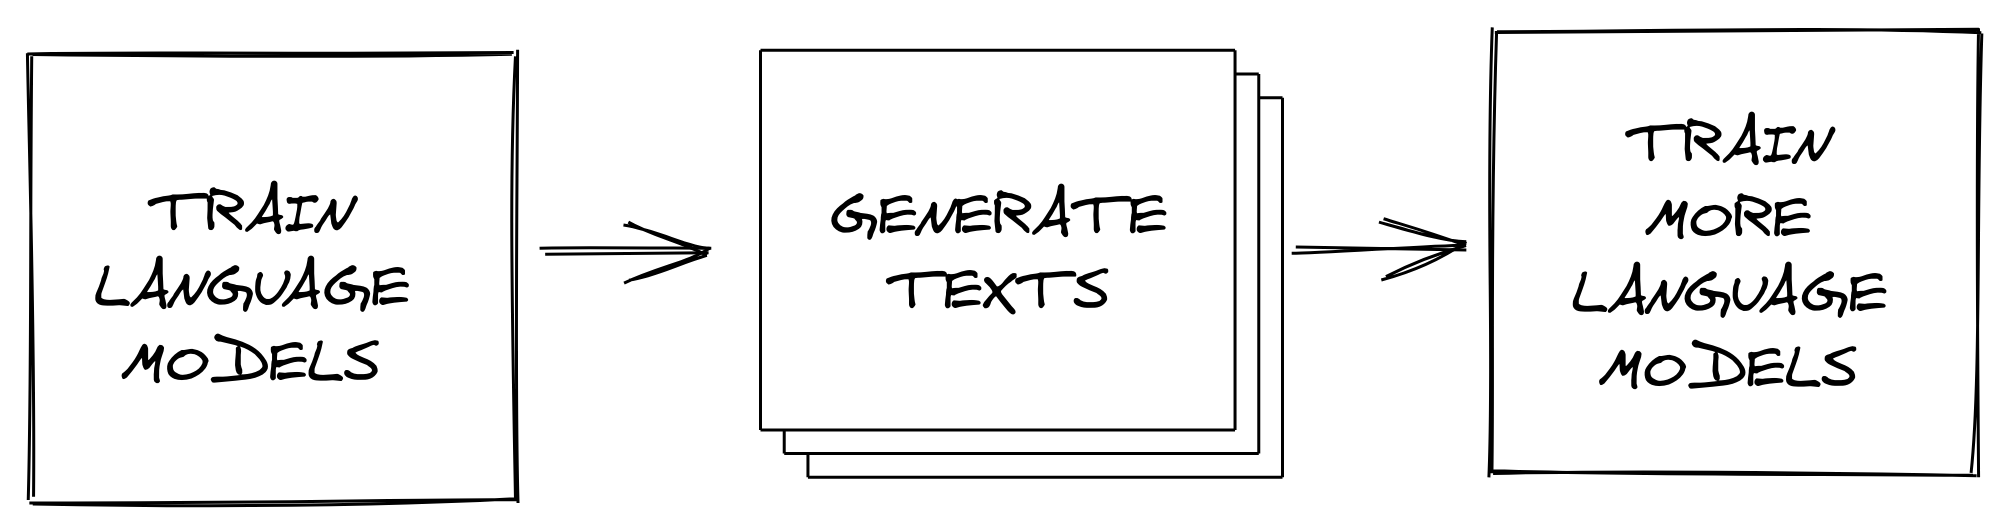
\includegraphics[width=\linewidth]{images/9.png}
\end{figure}
\end{frame}

%------------------------------------------------

\subsection{That's all}
\begin{frame}
\begin{figure}
	
\includegraphics[width=0.9\linewidth]{images/end.png}
\end{figure}
\end{frame}

%------------------------------------------------

%------------------------------------------------

\section{REFERENCES} 

\begin{frame}
\frametitle{}
\begin{thebibliography}{0}

\bibitem{transformer} ``Attention Is All You Need.`` arXiv preprint arXiv:1706.03762v5.

\bibitem{dilma} ``Differentiable Language Model Adversarial Attacks on Categorical Sequence Classifiers.`` arXiv preprint arXiv:2006.11078.

\bibitem{lstm} ``A Semi-supervised Approach to Generate the Code-Mixed Text using Pre-trained Encoder and Transfer Learning.`` Findings of the Association for Computational Linguistics: EMNLP 2020, pages 2267–2280

\bibitem{glue} ``DialoGLUE: A Natural Language Understanding Benchmark for Task-Oriented Dialogue.`` arXiv preprint arXiv:2009.13570v2.

\bibitem{xlm} Guillaume Lample, Alexis Conneau. 2019. ``Cross-lingual Language Model Pretraining.`` arXiv preprint arXiv:1901.07291.

\bibitem{xlmr} ``Unsupervised Cross-lingual Representation Learning at Scale.`` arXiv preprint arXiv:1911.02116v2.

\end{thebibliography}
\end{frame}

\end{document} 